\documentclass[../Main.tex]{subfiles}

\begin{document}

\npage{
    \begin{figure}[H]
        \begin{center}
            \def\svgwidth{\columnwidth}
            \input{Images/recorrido.pdf_tex}
        \end{center}
        \caption{Recorrido de una particula.}
        \label{fg:recorrido}
    \end{figure}
    }
{

    \section{Trabajo de una fuerza}
    Supongamos que queremos mover una caja, como la que aparece en la figura \ref{fg:recorrido},
    una distancia $\Delta \vec{r}$. Uno podria ejercerle una fuerza $\vec{F}$ y notaria 
    que para mover la caja depende de una serie de condiciones

    \begin{itemize}
        \item la distancia que uno quiere mover la caja;
        \item la magnitud de la fuerza;
        \item el angulo entre la fuerza y la distancia que uno quiere mover.
    \end{itemize}

    El ejemplo tipico que se utiliza para explicar el trabajo de una fuerza es 
    pensar en una particula que realiza un recorrido gracias a una fuerza( ver figura ())
    . Entonces sabemos que el trabajo de la fuerza se puede escribir de la siguiente
    manera

    \begin{equation}
        \partial W = \vec{F} \cdot \partial \vec{r}
        \label{eq:dtrabajo}
    \end{equation}
    donde 
    \begin{equation*}
        \partial \vec{r} = \partial r \cdot \hat{r} + r \cdot \theta \hat{\theta}
    \end{equation*}
    pero es solo para este caso porque me conviene verlo en polares.

    Si uno quisiera calcular el trabajo de una fuerza que realiza a lo largo de un
    desplazamiento, se hace de la siguiente forma
    \begin{equation*}
        W_{a \rightarrow b} = \int _a ^ b \vec{F} \cdot \partial \vec{r} \ .
    \end{equation*}

    Presentalo asi me deja insertar una duda y es lo siguiente
    \begin{equation*}
        \int _a ^ b \vec{F} \cdot \partial \vec{r} \ ? = ? \ \int _b ^ a \vec{F} \cdot \partial \vec{r} \ .
    \end{equation*}

    Respuesta corta, depende. Ese "depende" obvimente depende de la fuerza que
    estemos hablando.

    Con esta pregunta me permite introducir las fuerzas conservativas y las no
    conservativas.

    Las conservaticas son aquellas que su trabajo no depende del camnino recorrido
    para unir $a$ y $b$ sino de propiamente los puntos.

}

\npage{
Agregar figura donde hacen un circulo cerrado de a $\Rightarrow$ b
}
{
Ahora pensemos que pasa si una particula parte del punto $a$, avanza hasta el
punto $b$ y vuelve al punto $a$. Para ese caso especial se cumple lo
siguiente

\begin{equation*}
    W = W_{a \rightarrow b} + W_{b \rightarrow a}
\end{equation*}
\begin{equation*}
    \Downarrow
\end{equation*}
\begin{equation*}
    W = \int _{a_{C1}} ^ b \vec{F} \cdot \partial \vec{r} + \int _{b_{C2}} ^ a \vec{F} \cdot \partial \vec{r}
\end{equation*}
podemos usar un truco que se ve en el cbc y dar vuelta la integral del segundo
termino
\begin{equation*}
    W = \int _{a_{C1}} ^ b \vec{F} \cdot \partial \vec{r} - \int _{b_{C2}} ^ b \vec{F} \cdot \partial \vec{r}
\end{equation*}
\begin{equation*}
    \Downarrow
\end{equation*}
\begin{equation*}
    W = 0
\end{equation*}
ya que no importa el camino sino los puntos. Otra forma de escribir esto es 
\begin{equation*}
    \oint \vec{F} \cdot \partial \vec{r} = 0
\end{equation*}

El caso donde el trabajo varia dependiendo del camino se les dice fuerzas no
conservativa, un ejemplo de estas es el rozamiento o viscosa.

En general si la fuerza es una funcion de la distancia, esta sera conservativa.
Caso contrario, no lo es.
}

\npage{
    Hacer un dibujo, diria que el mismo que el anterior
}
{
    \section{Energia Cinetica}
    Supongamos un movil de masa $m$ que se ve afectada por una fuerza $\vec{F}$.
    Sabemos que su desplazamiento sera
    \begin{equation*}
        \partial \vec{r} = \vec{v} \cdot \partial t
    \end{equation*}

    entonces si pensamos en el la ecuacion \ref{eq:dtrabajo} y tenemos en cuenta la
    segunda ley de newton $\vec{F} = m \cdot \vec{a}$
    \begin{equation*}
        \partial W = \vec{F} \cdot \partial \vec{r} = m \cdot \vec{a} \cdot \vec{v} \cdot \partial t = m \cdot \frac{\partial \vec{v}}{\partial t} \cdot \vec{v} \cdot \partial t
    \end{equation*}
    obvimente se puede simplicar los diferenciales y se puede reescribir la derivada
    de la velocidad
    \begin{equation*}
        \partial W =  m \cdot \frac{1}{2} \cdot \partial \left( v^2 \right)
    \end{equation*}
    ahora podemos integrar en un punto $a$ y un punto $b$ 
    \begin{equation}
        W_{a \rightarrow b} = \int _a ^b m \cdot \frac{1}{2} \cdot \partial \left( v^2 \right) = \frac{1}{2} m \left( v_b^2 - v_a^2 \right) \ .
    \end{equation}

    Ahora podemos plantear el caso de que la fuerza esta trando de frenar al movil,
    entonces nos quedaria que $v_b^2 = 0$, la cuenta nos quederia
    \begin{equation}
        W_{a \rightarrow b} = - \frac{1}{2} m  \cdot v_a^2
    \end{equation}
    y se puede ver que la fueza le esta sacando energia al movil.

    A esto se lo conoce como \textit{Energia cinetica} y es la medida del trabajo
    que se puede extraer de un cuerpo en movimiento. A veces se lo escribe asi
    \begin{equation}
        T = \frac{1}{2} m  \cdot v^2
    \end{equation}
    siendo
    \begin{equation*}
        W_{a \rightarrow b} = T_b - T_a
    \end{equation*}

    A esto tambien se lo conoce como \textit{Teorema de las fuerzas vivas} ?

    Una ultima cosa y es que a $\vec{F}$ no le pedi nada en especial, osea que
    puede ser tanto conservativa o no.

}

\npage{
    % No hay imagenes en esta pagina
}
{
\section{Energia potencial}

Ahora si vamos a considerar que la fuerza es una conservativa. Existe una razon
de eso y es porque si recordamos que las fuerzas conservativas son funciones
de la posicion, osea que depende de la posicion, podemos decir lo siguiente
\begin{equation*}
     W_{x_0 \rightarrow x} = \int _{x_0}^x \vec{F} \cdot \partial \vec{r} = - \left[ V(x) - V(x_0) \right]
\end{equation*}
el $V(x)$ es lo que se conoce como potencial y es una parte de la energia
mecanica. Una forma mejor de ver la expresion como funcion de la posicion es
la siguiente
\begin{equation*}
     V(x) = - \int _{x_0}^x \vec{F} \cdot \partial \vec{r} + V(x_0)
\end{equation*}
$V(x_0)$ es una constante y en general se lo conoce como nivel de energia. En
si no es importante pero si es importante establecer un nivel de energia para
poder comparar. En muchas ocasiones se arreglan los terminos para que el nivel
de energia sea cero u otra espresicion que simplifique el resultado de la
integral.

\section{Una forma general de la energia mecanica}

Voy a dar una forma general que a mi me gusta porque mezcla todo y ademas es
util, al menos para mi, a la hora de resolver ejercicios. Partamos de una
particula que se ve afectada por un una fuerza y tienen una velocidad $\vec{v}$.
Lo primero que uno siempre hacer es presentar la segunda ley de newton

\begin{equation*}
     m \cdot \vec{a} = \sum{\vec{F}}
\end{equation*}
ahora, la sumatorio de fuerzas sabes que se puede dividir en dos grupos, que sea
la suma de las fuerzas conservativas y la sumatoria de las fuerzas no conserva
tivas. Ademas, voy a ver a reemplazar la aceleracion con lo siguiente

\begin{equation*}
    \vec{a} = \frac{\partial \vec{v}}{\partial t} = \frac{\partial \vec{v}}{\partial t} \cdot \frac{\partial \vec{r}}{\partial \vec{r}} = \frac{\partial \vec{r}}{\partial t} \cdot \frac{\partial \vec{v}}{\partial \vec{r}} = \vec{v} \cdot \frac{\partial \vec{v}}{\partial \vec{r}} = \frac{1}{\partial \vec{r}} \cdot \frac{1}{2} \cdot \partial \left( v^2 \right)
\end{equation*}

}

\npage{
}
{

Ahora si, podemos reemplazar en la ecuacion de newton

\begin{equation*}
     m \cdot \frac{1}{\partial \vec{r}} \cdot \frac{1}{2} \cdot \partial \left( v^2 \right) = \vec{F}^{C} + \vec{F}^{NC}
\end{equation*}
\begin{equation*}
     \Downarrow
\end{equation*}
\begin{equation*}
     m \cdot \frac{1}{2} \cdot \partial \left( v^2 \right) = \vec{F}^{C} \cdot \partial \vec{r} + \vec{F}^{NC} \cdot \partial \vec{r}
\end{equation*}
integramos en ambos lados
\begin{equation*}
     \int_{v_0^2}^{v^2} m \cdot \frac{1}{2} \cdot \partial \left( v^2 \right) = \int_{\vec{r_0}}^{\vec{r}} \vec{F}^{C} \cdot \partial \vec{r} + \int_{\vec{r_0}}^{\vec{r}} \vec{F}^{NC} \cdot \partial \vec{r}
\end{equation*}
\begin{equation*}
     \Downarrow
\end{equation*}
\begin{equation*}
    \frac{1}{2} \cdot m \cdot v^2 - \frac{1}{2} \cdot m \cdot v_0^2 = E_c - E_{c_0}= - \left[ V(\vec{r}) - V(\vec{r}_0) \right] + W_{x_0 \rightarrow x}^{NC}
\end{equation*}
\begin{equation*}
     \Downarrow
\end{equation*}
\begin{equation*}
    E_c - E_{c_0} + V(\vec{r}) - V(\vec{r}_0) = W_{x_0 \rightarrow x}^{NC}
\end{equation*}
\begin{equation*}
     \Downarrow
\end{equation*}
\begin{equation}
    \left[ E_c + V(\vec{r}) \right] - \left[E_{c_0} + V(\vec{r}_0) \right] = W_{x_0 \rightarrow x}^{NC}
    \label{eq:deltae}
\end{equation}
el primer parentesis es la energia mecanica para un instante generico y el segundo
parentesis es la energia mecanica en un instante inicial. Lo bueno de esta
ultima exprecion es la facilidad que brinda para reconcer cuando la energia
mecanica se conserva y es cuando el trabajo de las fuerzas no conservativas
sea cero. El hecho que sea sea cero quiere decir que tanto la cinetica como
la potencial se van a equilibrar.
Una forma de ver la energia mecanica para un instante dado es la siguiente
\begin{equation*}
    H =  E_c + V(\vec{r})
\end{equation*}

\section{Un par de ejericios}


\ejem{Caida libre}{Supongamos una pelota de masa $m$ parte de reposo y se deja
cae una altura $h$. Cual es la velocidad final?}

Primero se plantea la segunda ecuacion de Newton para este cuerpo

\begin{equation*}
    m \cdot \vec{a} = \sum \vec{F} = m \cdot \vec{g} \ .
\end{equation*}

}

\npage{
}
{

En este caso es bastante sencilla porque solo esta la fuerza peso y no hay otra
involucrada. Voy hacer los mismos pasos que hice para llegar a la expresion \ref{eq:deltae}
y no voy a simplificar las masas para que me quede la expresion generica de la
energia
\begin{equation*}
    m \cdot \frac{1}{\partial \vec{r}} \cdot \frac{1}{2} \cdot \partial \left( v^2 \right) = m \cdot \vec{g}
\end{equation*}
\begin{equation*}
    \Downarrow
\end{equation*}
\begin{equation*}
    \frac{1}{2} \cdot m \cdot \partial \left( v^2 \right) = m \cdot \vec{g} \cdot \partial \vec{r}
\end{equation*}
\begin{equation*}
    \Downarrow
\end{equation*}
\begin{equation*}
    \int_{v_0^2}^{v^2} \frac{1}{2} \cdot m \cdot \partial \left( v^2 \right) = \int_{\vec{r}_0}^{\vec{r}}m \cdot \vec{g} \cdot \partial \vec{r}
\end{equation*}
\begin{equation*}
    \Downarrow
\end{equation*}
\begin{equation*}
    \frac{1}{2} \cdot m \cdot v^2 - \frac{1}{2} \cdot m \cdot v_0^2 = m \cdot \vec{g} \cdot \left( \vec{r} - \vec{r_0} \right) \ .
\end{equation*}
Ahora nos toca reemplzar con los datos que tenemos. Si ponemos nuestros ejes de
refercia en el momento que la masa parte tenemos que $\vec{r}_0 = 0 \cdot \hat{z}$
y como queremos saber a que velocidad llega en $h$ podemos poner $\vec{r} = h \cdot \hat{z}$.
Ademas sabemos que parte de reposo por lo que $v_0^2 = 0$ y que la gravadad 
$\vec{g} = +|g| \cdot \hat{z}$ por nuestros ejes. Ahora si, reemplzamos
\begin{equation*}
    \frac{1}{2} \cdot m \cdot v_f^2 - \frac{1}{2} \cdot m \cdot 0^2 = m \cdot |g| \cdot \hat{z} \cdot \left( h \cdot \hat{z} - 0 \cdot \hat{z} \right)
\end{equation*}
\begin{equation*}
    \Downarrow
\end{equation*}
\begin{equation*}
    \frac{1}{2} \cdot m \cdot v_f^2 = m \cdot |g| \cdot h
\end{equation*}
\begin{equation*}
    \Downarrow
\end{equation*}
\begin{equation*}
    \cdot v_f^2 = 2 \cdot |g| \cdot h \Rightarrow |v_f| = \sqrt{2 \cdot |g| \cdot h} \ .
\end{equation*}

Para el caso de un tiro vertical es analogo el resultado.

\ejem{Masa con resorte}{Supongamos una masa que esta atada a un resorte de una
constante elastica $k$ y con una longitud natural $l_0$. Describa y grafique
el potencial de la fuerza elastica.}

Para este tipo de ejercicios lo que uno hace es simplemente tratar con las 
fuerzas conservaticas, no vamos a tener en cuenta la parte de cinetica. Como la
una fuerza conservativa que permanece en el sistema es el resorte, vamos a
describir ese potencial.

}

\npage{
}
{

\begin{equation*}
    \vec{F_k} (x) = - k \left( x - l_0 \right) \hat{x}
\end{equation*}
sabemos que el trabajo de la fuerza se puede escribir como
\begin{equation*}
    \partial W = \vec{F_k} (x) \cdot \partial \vec{r}
\end{equation*}
como solo se puede mover en $\hat{x}$ se puede decir que
\begin{equation*}
    \vec{r} = x \cdot \hat{x} \Rightarrow \partial \vec{r} = \partial x \cdot \hat{x}
\end{equation*}
entonces si reemplazamos en el trabajo
\begin{equation*}
    \partial W = \vec{F_k} (x) \cdot \partial \vec{r} = - k \left( x - l_0 \right) \hat{x} \cdot \partial x \cdot \hat{x}
\end{equation*}
\begin{equation*}
    \Downarrow
\end{equation*}
\begin{equation*}
    \partial W = - k \cdot x \cdot \partial x + k \cdot l_0 \cdot \partial x
\end{equation*}
ahora podemos integrar en ambos lados solo que en la izquierda de la igualdad
vamos a poner el potencial
\begin{equation*}
    \int_{W_0}^W \partial W = \int_{x_0}^{x} - k \cdot x \cdot \partial x + \int_{x_0}^{x} k \cdot l_0 \cdot \partial x
\end{equation*}
\begin{equation*}
    \Downarrow
\end{equation*}
\begin{equation*}
    - \left[ V(x) - V(x_0) \right] = - k \cdot \frac{1}{2} \cdot \left( x ^2 |_{x_0}^{x} \right) + k \cdot l_0 \cdot \left( x |_{x_0}^{x} \right)
\end{equation*}
\begin{equation*}
    \Downarrow
\end{equation*}
\begin{equation*}
    - \left[ V(x) - V(x_0) \right] = - k \cdot \frac{1}{2} \cdot \left(x^2 - x_0^2 \right) + k \cdot l_0 \cdot \left( x - x_0 \right)
\end{equation*}
\begin{equation*}
    \Downarrow
\end{equation*}
\begin{equation*}
    V(x) - V(x_0) = k \cdot \frac{1}{2} \cdot \left(x^2 - x_0^2 \right) - k \cdot l_0 \cdot \left( x - x_0 \right)
\end{equation*}
\begin{equation*}
    \Downarrow
\end{equation*}
\begin{equation*}
    V(x) = k \cdot \frac{1}{2} \cdot \left(x^2 - x_0^2 \right) - k \cdot l_0 \cdot \left( x - x_0 \right) + V(x_0) 
\end{equation*}
de aca se puede ver si yo tomo $x_0 = l_0$ y $V(x_0) = 0$ se me simplifica la
cuenta, ademas voy llevar la expresion para que la x me quede aparte
\begin{equation*}
    V(x) = k \left[ \frac{1}{2} \cdot \left(x^2 - l_0^2 \right) - l_0 \cdot \left( x - l_0 \right) \right]
\end{equation*}
\begin{equation*}
    \Downarrow
\end{equation*}
\begin{equation*}
    V(x) = k \left[ \frac{1}{2} \cdot x^2 - \frac{1}{2} \cdot l_0^2 - l_0 \cdot x + l_0^2 \right]
\end{equation*}

}

\npage{
}
{

\begin{equation*}
    V(x) = k \left[ \frac{1}{2} \cdot x^2 - l_0 \cdot x + \frac{1}{2} l_0^2 \right]
\end{equation*}
esto se puede ver como un binomio al cuadrado
\begin{equation*}
    V(x) = k \cdot \frac{1}{2} \left[ x^2 - 2 \cdot l_0 \cdot x + l_0^2 \right]
\end{equation*}
\begin{equation*}
    \Downarrow
\end{equation*}
\begin{equation*}
    V(x) = \frac{k}{2} \left( x - l_0 \right)^2
\end{equation*}
Si uno graficara esto obtendria lo siguiente
\begin{figure}[H]
    \begin{center}
        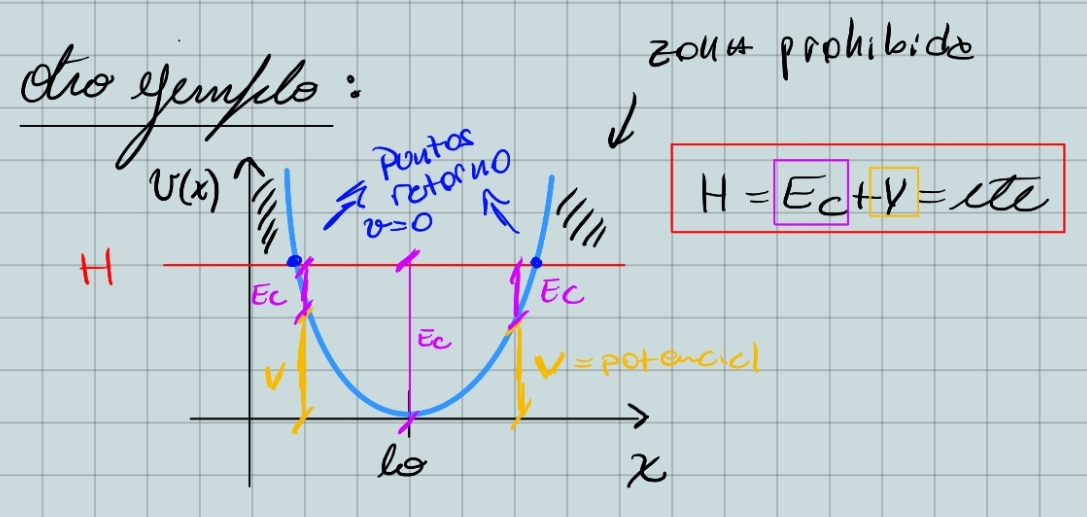
\includegraphics[scale=0.5]{Images/potencial_resorte.jpg}
    \end{center}
\end{figure}

\ejem{El problema de kepler}{En si lo pongo porque es un problema que al menos
en el final de capuzzi suele aparecer entonces lo voy a desarrollar. Este 
empieza asi, Estudie el problema de Kepler para el sistema Sol (de masa $M$)
- Tierra (de masa $m << M$)
\begin{itemize}
    \item Exprese el impulso lineal, el momento angular y la energia mecanica
    \item Encontrar que magnitudes se conservan
    \item Encontrar y graficar el potencial efectivo
\end{itemize}
}

Empecemos describiendo las fuerzas que sienten cada uno. Para la masa $M$ tengo
que siente la fuerza de atraccion de la masa $m$
\begin{equation*}
    \vec{F}_{Mm} = G \cdot \frac{m \cdot M}{\vec{r} \ ^2} \cdot \hat{r}_{Mm}
\end{equation*}
donde $\hat{r}_{Mm}$ es un vector unitario que me invente pero que parte de la
masa $M$ y apunta a la masa $m$ y $\vec{r}$ es la distancia entre ellas.

}

\npage{
    % No hay imagenes en esta pagina
}
{
    Para el caso de la masa de la masa $m$ le pasa algo similar

    \begin{equation*}
        \vec{F}_{mM} = G \cdot \frac{M \cdot m}{\vec{r} \ ^2} \cdot \hat{r}_{mM}
    \end{equation*}
    donde $\hat{r}_{mM}$ es un vector unitario que parte de la masa $m$ y apunta a
    la masa $M$ y $\vec{r}$ es la distancia entre ellas.

    Una relacion que sale de forma inmediata es es la siguiente 
    \begin{equation*}
        \hat{r}_{Mm} = - \hat{r}_{mM}
    \end{equation*}
    esto es valido para todo el movimiento ya que siempre vas a estar apuntandose
    de forma contraria. Ahora voy a escribir las ecuaciones de Newton y voy a
    quedarme con esa relacion de los versores que me invente para reemplazarlo.

    Para la masa $M$ tengo que
    \begin{equation*}
        M \cdot \vec{a}_M = \vec{F}_{Mm} = G \cdot \frac{m \cdot M}{\vec{r} \ ^2} \cdot \hat{r}_{Mm}
    \end{equation*}
    \begin{equation*}
        \Downarrow
    \end{equation*}
    \begin{equation*}
        M \cdot \vec{a}_M = G \cdot \frac{m \cdot M}{\vec{r} \ ^2} \cdot \left( - \hat{r}_{mM} \right) \ .
    \end{equation*}

    Y para la masa $m$ tengo
    \begin{equation*}
        m \cdot \vec{a}_m = G \cdot \frac{M \cdot m}{\vec{r} \ ^2} \cdot \hat{r}_{mM} \ .
    \end{equation*}

    Una vez establecidas ambas ecuaciones voy a sumarlas
    \begin{equation*}
        m \cdot \vec{a}_m + M \cdot \vec{a}_M = G \cdot \frac{M \cdot m}{\vec{r} \ ^2} \cdot \hat{r}_{mM} - G \cdot \frac{m \cdot M}{\vec{r} \ ^2} \cdot \hat{r}_{mM}
    \end{equation*}
    \begin{equation*}
        \Downarrow
    \end{equation*}
    \begin{equation*}
        m \cdot \vec{a}_m + M \cdot \vec{a}_M = 0
    \end{equation*}
    \begin{equation*}
        \Downarrow
    \end{equation*}
    \begin{equation*}
        m \cdot \frac{\partial \vec{v}_m}{\partial t} + M \cdot \frac{\partial \vec{v}_M}{\partial t} = 0
    \end{equation*}
    \begin{equation*}
        \Downarrow
    \end{equation*}
    \begin{equation*}
        \frac{\partial }{\partial t} \left( m \cdot \vec{v}_m + M \cdot \vec{v}_M \right) = 0 = \frac{\partial \vec{P}}{\partial t}
    \end{equation*}
    de aca concluyo que que el impulso lineal se conserva por la falta de fuerzas
    externas.

    No solo eso, sino que tambien puedo decir que el centro de masa se mueve como
    un MRU porque a esta expresion puedo multiplicar las masas y obtengo la derivada
    de la velocidad centro de masa respecto del tiempo

}

\npage{
    % No hay imagenes en esta pagina
}
{

    \begin{equation*}
        \frac{\partial }{\partial t} \left( \frac{m \cdot \vec{v}_m + M \cdot \vec{v}_M}{m + M} \right) = \frac{\partial V_{CM}}{\partial t} = 0 \ .
    \end{equation*}

    Ahora tendria que ver el impulso angular y para eso vamos a pensar para eso
    necesito un punto de donde medirlo. Para eso voy a usar el centro de masa

    \begin{equation*}
        \vec{r}_{CM} = \frac{m \cdot \vec{r}_m + M \cdot \vec{r}_M}{m + M}
    \end{equation*}

    Ademas tenemos que la distancia relativa entre ellos es

}

\end{document}
